\begin{figure}[!t]
  \centering
  \begin{minipage}[t]{\columnwidth}
    \centering
    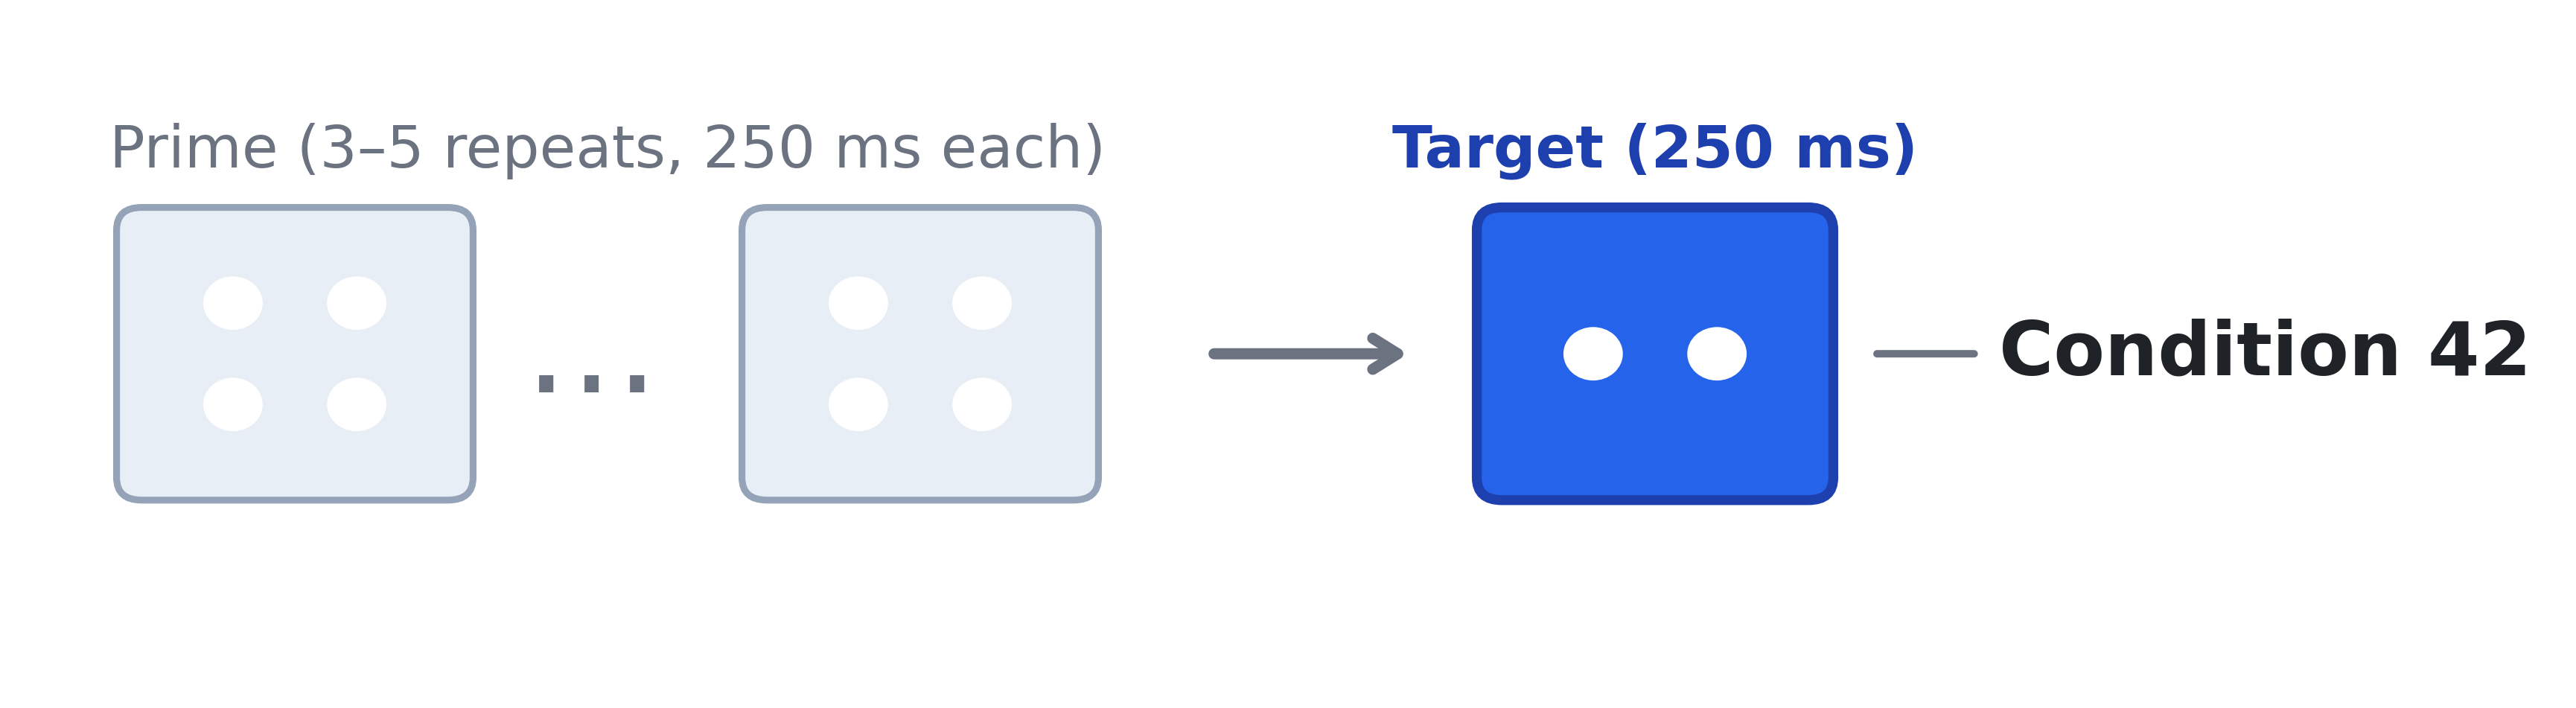
\includegraphics[width=0.85\columnwidth]{media/trial_structure.png}
    \vspace{-1mm}
    \subcaption{Single-trial structure. Three to five identical prime
    images precede a target that differs in numerosity. Condition codes
    denote the prime-target pair (e.g., ``42'' = prime 4, target 2).}
    \label{fig:trial-structure}
  \end{minipage}

  \vspace{4pt}

  \begin{minipage}[t]{\columnwidth}
    \centering
    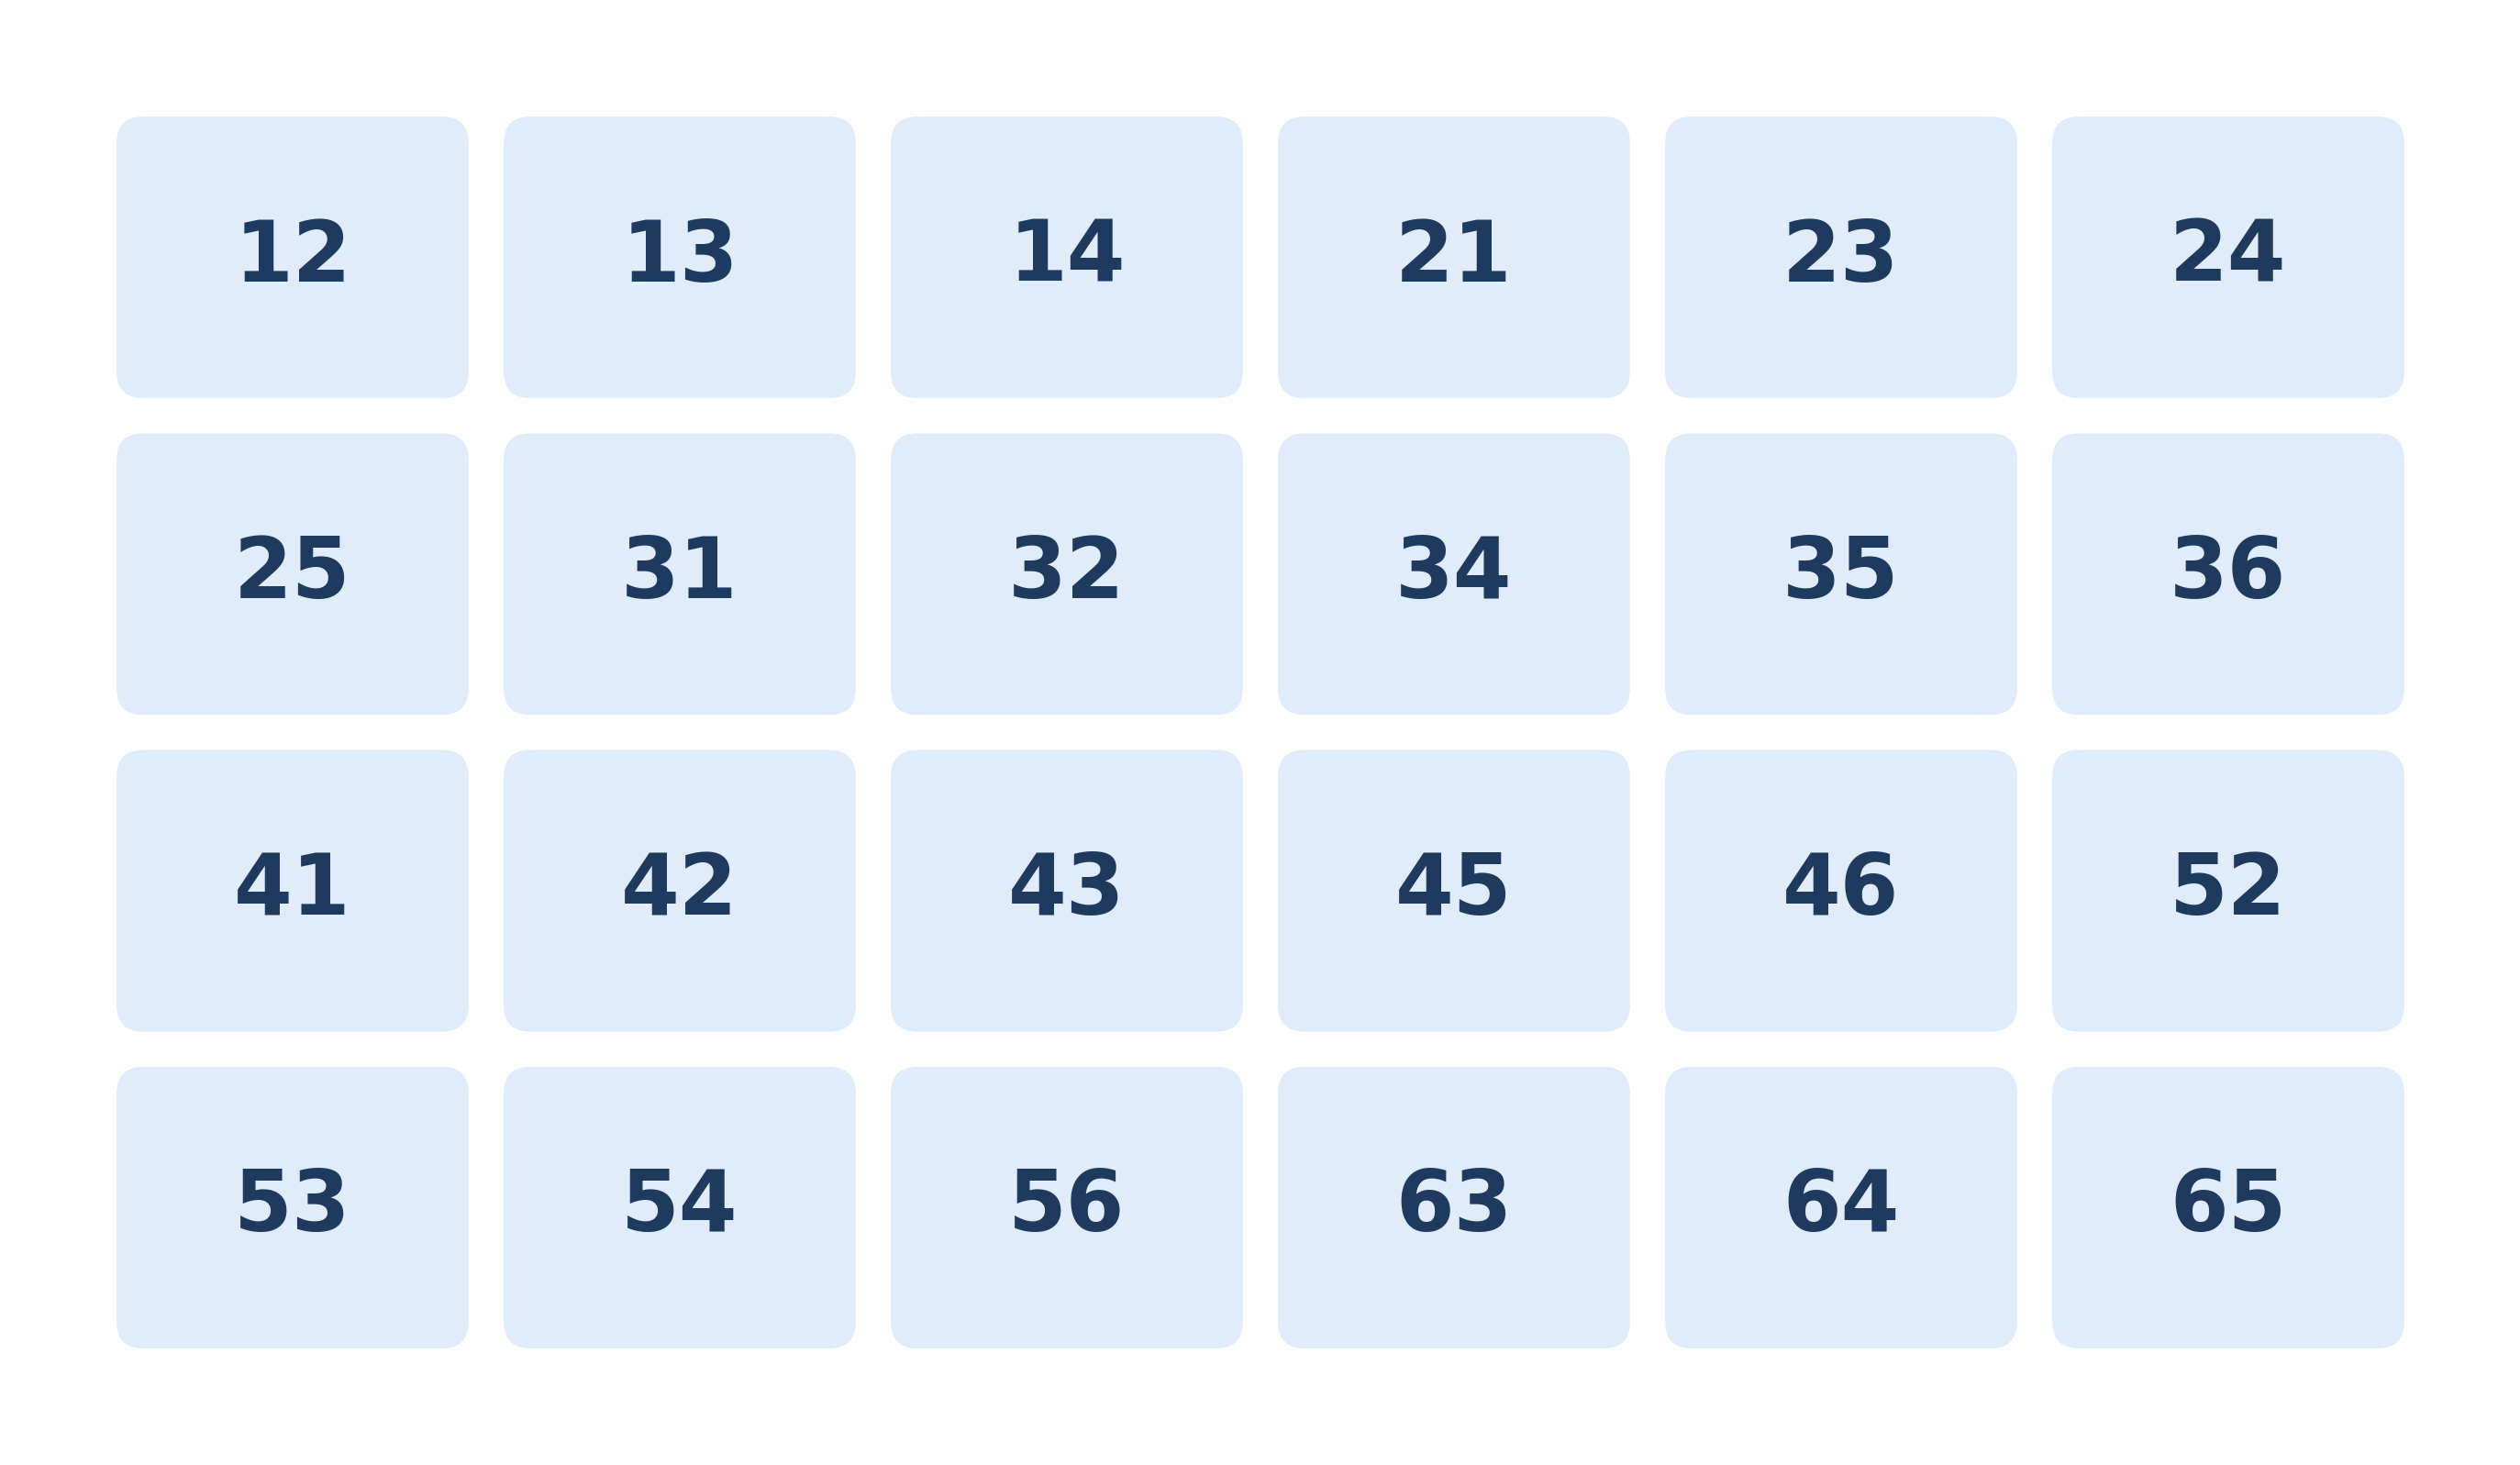
\includegraphics[width=0.75\columnwidth]{media/conditions-24.png}
    \vspace{-1mm}
    \subcaption{All 24 prime-target change conditions used in this
    study. Prime and target differ by 1-3 items within the 1-6 range.}
    \label{fig:condition-matrix}
  \end{minipage}

  \vspace{4pt}

  \begin{minipage}[t]{\columnwidth}
    \centering
    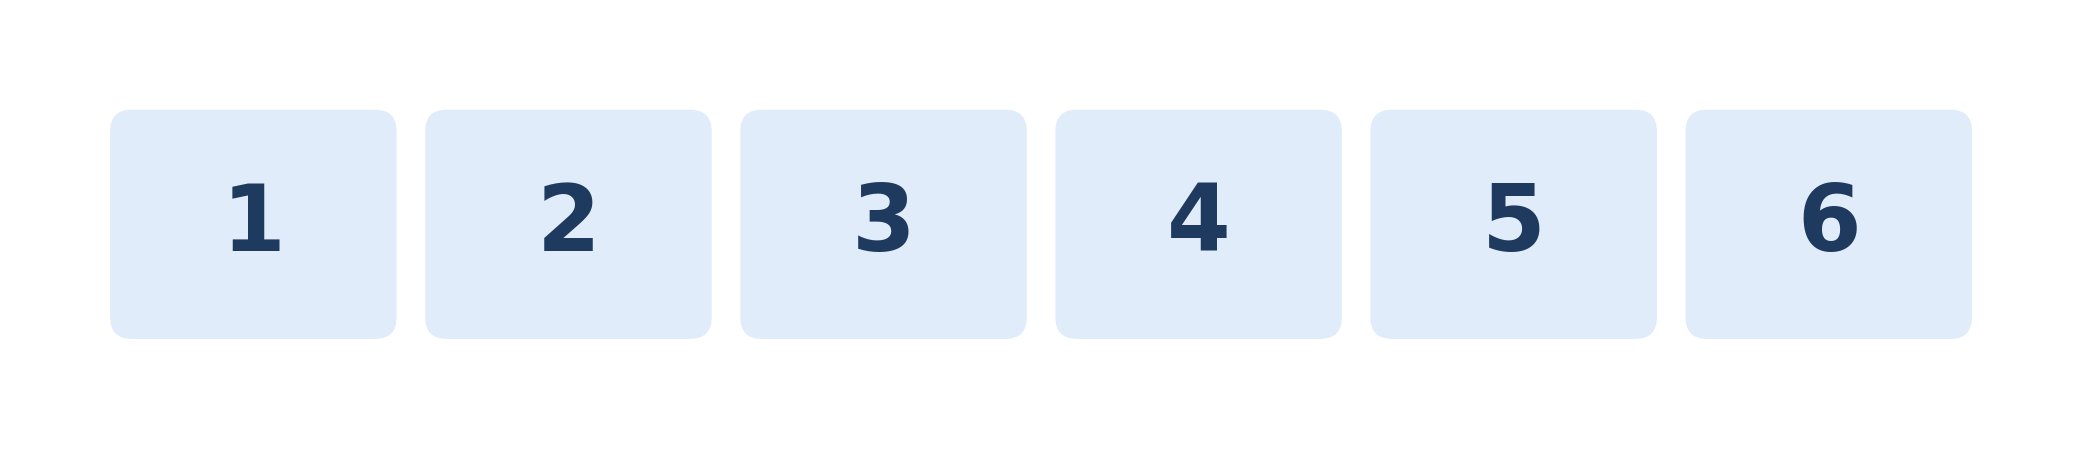
\includegraphics[width=0.70\columnwidth]{media/conditions-6.png}
    \vspace{-1mm}
    \subcaption{Whole-epoch target numerosities (1-6), obtained by
    collapsing across prime identity in (b).}
    \label{fig:condition-6}
  \end{minipage}
  \caption{Task design.}
  \label{fig:task-design}
\end{figure}
